\chapter{Mengenal Kecerdasan Buatan dan Scikit-Learn}
\section{Teori}
Praktek teori penunjang yang dikerjakan :
\begin{enumerate}
\item
Buat Resume Definisi, Sejarah dan perkembangan Kecerdasan Buatan, dengan bahasa yang mudah dipahami dan dimengerti. Buatan sendiri bebas plagiat[hari ke 1](10)
\subsection{Definisi Kecerdasan Buatan}
\begin{enumerate}
\item Menurut John McCarthy (1956), Artifical Intelligence adalah suatu sistem komputer yang terbentuk untuk mengetahui dan memodelkan proses-proses berpikir manusia dan mendesain mesin agar dapat menirukan perilaku manusia. 
\item Menurut Rich dan Knight (1991, p3), Artifical Intelligence merupakan ilmu yang mempelajari bagaimana membuat sebuah komputer dapat mengerjakan sesuatu yang masih lebih baik dikerjakan manusia.  
\item Menurut Rolston (1988, p 15), Artificial Intelligence merupakan solusi berbasis komputer terhadap masalah yang ada, dengan menggunakan aplikasi yang mirip sesuai dengan proses berpikir menurut manusia.
\item Menurut Setiawan (1933, p 1), Artificial Intelligence dapat diartikan sebagai cabang ilmu komputer yang mempelajari tentang otomatisasi tingkah laku cerdas.
\end{enumerate}
\noindent
Jadi, dapat disimpulkan bahwa Kecerdasan Buatan atau Artifical intelligence(AI) adalah  suatu ilmu komputer yang membuat komputer(mesin) dapat menirukan perilaku manusia dengan baik. 
\subsection{Sejarah dan perkembangan Kecerdasan Buatan}
Istilah Artificial Intelligence dikemukakan untuk pertama kali tahun 1956 dalam Konferensi Dartmouth sehingga mulai saat itu Artifical Intelligence terus dikembangkan sebab berbagai penelitian mengenai teori-teori dan prinsip-prinsipnya juga terus berkembang. Istilah Artificial Intelligence baru muncul tahun 1956, tetapi teori-teori sudah muncul sejak tahun 1941. 
\hfill\break
\noindent
Berikut tahapan-tahapan sejarah perkembangan kecerdasan buatan:
\begin{enumerate}
\item Era Komputer Elektronik (1941)
\hfill\break
1941 merupatah tahun yang telah ditemukan alat penyimpanan dan pemrosesan informasi yang diberi nama komputer elektronik yang dikembangkan di USA dan Jerman dan oleh karenanya komputer pertama ini memerlukan ruangan yang luas dan ruang AC yang terpisah. Saat itu komputer melibatkan konfigurasi ribuan kabel untuk bisa menjalankan program. Tahun 1943, berhasil dibuat sebuah komputer yang mampu menyimpan program sehingga membantu pekerjaan dalam memasukkan program menjadi lebih mudah. Dan penemuan ini menjadi dasar pengembangan untuk program yang mengarah pada artificial intelligence.
\item Masa-Masa Persiapan AI (1943 - 1956) 
\hfill\break
Warren McCulloch dan Walter Pitt pada tahun 1943 mengemukakan terdapat 3 hal dalam masa persiapan yaitu pertama pengetahuan fisiologi dasar dan fungsi sel syaraf dalam otak,kedua analisis formal tentang logika proposisi, dan ketiga teori komputasi Turing. Mereka berhasil membuat sebuah tiruan model sel syaraf, tiruan yang dimana setiap sel syaraf digambarkan sebagai 'on' dan 'off'. Mereka menunjukkan bahwa setiap fungsi mampu dihitung melalui jaringan sel syaraf dan semua hubungan logis dapat diimplementasikan dengan struktur jaringan sederhana.
\hfill\break
Pada tahun 1950, Nobert Wiener membuat sebuah penelitian mengenai prinsip-prinsip tentang teori feedback. Contoh yang terkenal adalah thermostat. Penemuan ini juga merupakan awal dari perkembangan Artificial Intelligence. 
\hfill\break
Tahun 1956, John McCarthy meyakinkan Minsky, Claude Shannon dan Nathaniel Rochester untuk membantunya dalam sebuah penelitian dengan beberapa ilmuan bidan Otomata, Jaringan Syaraf dan pembelajaran intelijensia. Mereka mengerjakan proyek tersebut selama 2 bulan di Dartsmouth. Hasilnya yang didapatkan adalah program yang mampu berpikir non-numerik dan menyelesaikan masalah pemikiran, disebut Principia Mathematica. Hal ini menjadi McCarthy disebut sebagai bapak kecerdasan buatan.
\item Awal Perkembangan AI(1952-1969)
\hfill\break
Pada tahun-tahun pertama perkembangannya, Artificial Intelligence mengalami banyak kesuksesan. Diawali dengan kesuksesan Newell dan Simon dengan sebuah program yang diberi nama General Problem Solver. Program ini dirancang digunakan untuk menyelesaikan sebuah masalah secara manusiawi.
\hfill\break
McCarthy di MIT Al Lab Memo No.1 mendefinisikan bahasa pemrograman tingkat tinggi yaitu LISP, yang saat ini telah mendominasi pembuatan program-program Artificial Intelligence pada Tahun 1958. Kemudian McCarthy membuat sebuah program yang diberi nama Programs with Common Sense. Di dalam program tersebut, dibuat rancangan yang digunakan untuk menggunakan pengetahuan dalam mencari sebuah solusi. 
\hfill\break
Nathaniel Rochester dari IBM dan mahasiswa-mahasiswanya berhasil mengeluarkan program Artifical Intelligence yaitu Geometry Theorm Prover pada tahun 1959. Program ini mampu mengeluarkan teorema dengan menggunakan aksioma-aksioma yang ada.
\hfill\break
Pada tahun 1963, program yang dibuat James Slagle telah berhasil menyelesaikan masalah integral tertutup untuk mata kuliah Kalkulus.
\hfill\break
Program analogi yang dibuat Tom Evan pada tahun 1986 mampu menyelesaikan masalah analogi geometris yang ada pada tes IQ pada.
\item Perkembangan Kecerdasan Buatan Melambat (1966-1974)
\hfill\break
Perkembangan Artificial Intelligence melambat yang disebabkan adanya 3 kesulitan utama, yaitu:
\begin{enumerate}
\item Program-program Artificial Intelligence yang bermunculan hanya mengandung sedikit atau bahkan tidak mengandung sama sekali pengetahun(knowledge) pada subjeknya. Program-program kecerdasan buatan berhasil hanya karena manipulasi sederhana. Sebagai contoh yaitu Weizenbaum's ELIZA program(tahun 1956) berhasil melakukan percakapan serius dengan berbagai topik, yang sebenernya hanyalah peminjaman manipulasi kalimat-kalimat yang sudah diketikkan oleh manusia.
\item Banyak masalah yang harus diselesaikan oleh kecerdasan bautan.
\item Ada beberapa batasan ada struktur dasar yang digunakan untuk menghasilkan perilaku intelijensia.
\end{enumerate}
\item Sistem Berbasis Pengetahuan (1969-1979)
\hfill\break
Pengetahuan adalah kekuatan pendukung kecerdasan buatan. Dibuktikan dengan program yang dibuat  Ed Feingenbaum, Bruce Buchanan dan Joshua Lederberg, membuat sebuah program untuk memecahkan suatu masalah struktur molekul dari informasi yang sumbernya diperoleh melalui spectrometer massa. Pogram ini dinamakan Dendral Programs yang berfokus dengan segi pengetahuan kimia. Dari segi diagnose medis jugaa telah ditemukannya, yaitu Sau Amarel dalam proyek Computer in Biomedicine.
\item Kecerdasan Buatan menjadi sebuah industri (1980-1988)
\hfill\break
Industrialisasi Artificial Intelligence diawali dengan ditemukannya sistem pakar yang didefinisikan R1 yang mampu mengkonfigurasi suatu sistem-sistem komputer baru. Tahun 1982, Program mulai dioperasikan ke Digital Equipment Corporation(DEC), McDermott.
\hfill\break
Pada tahun 1986, R1 telah berhasil menghemat US\$40 juta pertahun.
\hfill\break
Pada taun 1988, kelompok Artificial Intelligence di DEC menjalankan 40 sistem pakar. Hampir semua perusahaan besar di USA mempunyai divisi Artificial Intelligence. Sehingga perusahaan yang sejak tahun 1982 hanya menghasilkan beberapa juta US dolar per tahun meingkat menjadi 2 milliar US dolar per tahun pada tahun 1988.
\item Kembalinya Jaringan Syaraf Tiruan (1986-Sekarang)
\hfill\break
Bidang ilmu komputer menolak adanya jaringan syaraf tiruan dengan diterbitkannya sebuah buku "Perceptrons" karangan Minsky dan Papert, sehingga sampai saat ini mereka masih mempelajari bidang ilmu dari sudut pandang yang lainnya, yaitu fisika. Para ahli fisika seperti Hopefield(pada tahun 1982) menggunakan sebuah teknik-teknik mekanika statistika untuk menganalisa sifat-sifat penyimpanan dan optimasi pada sebuah jaringan syaraf. Para ahli psikologi, David Rumelhart dan Geoff Hinton, melanjutkan penelitian mengenai model sebuah jaringan syaraf tiruan pada memori.
\hfill\break
Terdapat 4 kelompok riset yang menemukan kembali algoritma belajar propagasi balik (Back-Propagation Learning)pada tahun 1985. Algoritma ini berhasil diimplementasikan ke dalam suatu bidang ilmu komputer dan psikologi.
\end{enumerate}
\item
Buat Resume mengenai definisi supervised learning, klasifikasi, regresi dan unsupervised learning. Data set, training set dan testing set.[hari ke 1](10)
\begin{enumerate}
\item Definisi Supervised Learning
\hfill\break
Supervised Learning merupakan salah satu jenis yang populer untuk melakukan operasi machine learning dan banyak digunakan untuk data di mana ada pemetaan antara data input-output. Kumpulan data, untuk hal ini, diberi nama dengan label, artinya algoritma mengidentifikasi fitur secara eksplisit dan melakukan prediksi atau klasifikasi yang sesuai.
\begin{figure}[h]
	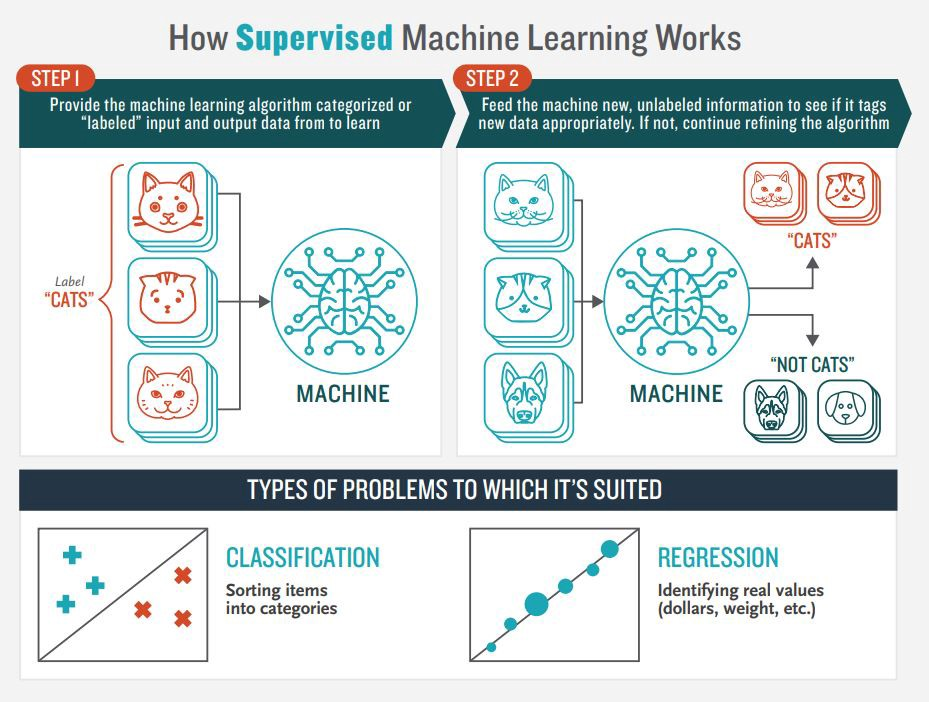
\includegraphics[width=1\textwidth]{figures/1184065/SupervisedLearning.jpeg}
	\centering
	\caption{Supervised Learning}
\end{figure}
\item Definisi Klasifikasi
\hfill\break
Classification merupakan suatu tindakan digunakan untuk memberikan kelompok pada setiap keadaan. Setiap keadaan berisi sekelompok atribut, salah satunya yaitu class attribute. Metode ini butuh untuk menemukan model yang mampu menjelaskan class atribute sebagai fungsi dari input attribute.
\begin{figure}[h]
	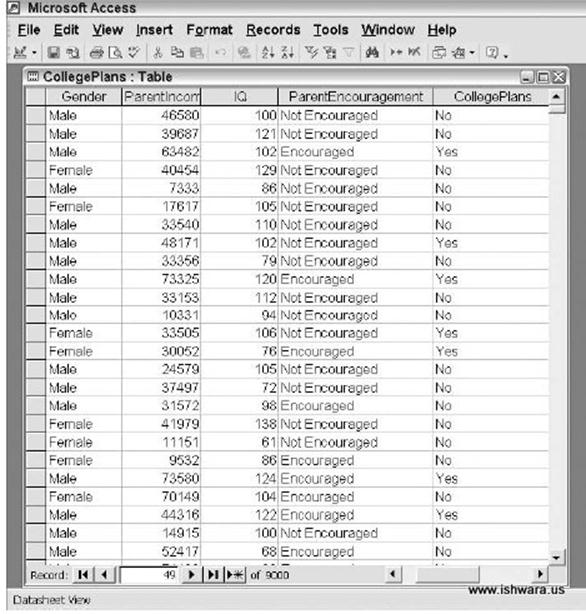
\includegraphics[width=1\textwidth]{figures/1184065/Classification.jpg}
	\centering
	\caption{Classification}
\end{figure}
\hfill\break
Class adalah attribute CollegePlans yang memiliki isi dengan dua pernyataan, Yes dan No.
\item Definisi Regresi
\hfill\break
Metode Regression hampir sama dengan metode Classification, bedanya karena  metode regression tidak bisa untuk mencari pola yang dijabarkan untuk menjadi class (kelas). 
\hfill\break
Metode Regression memiliki tujuan untuk mencari pola dan menentukan sebuah nilai numerik. Teknik Linear Line-Fitting sederhana adalah contoh dari Regression, hasilnya merupakan sebuah fungsi yang difungsikan untuk menentukan hasil berdasarkan nilai dari input. 
\hfill\break
Regression digunakan untuk memecahkan banyak problem bisnis, contohnya pertama memperkirakan metode distribusi, kedua kapasitas distribusi, ketiga musim dan kemudian untuk memperkirakan kecepatan angin berdasarkan temperatur, tekanan udara, dan kelembapan.
\item Definisi Unsupervised Learning
\hfill\break
Unsupervised Learning merupakan tipe algoritma machine learning, digunakan untuk menarik kesimpulan dari sebuah dataset dan metode ini hanya mempelajari suatu data berdasarkan kedekatannya atau disebut dengan clustering. Metode Unsupervised Learning yang paling umum ialah analisis cluster,yang berfungsi pada analisa data untuk mencari pola-pola tersembunyi atau pengelompokan data.
\begin{figure}[h]
	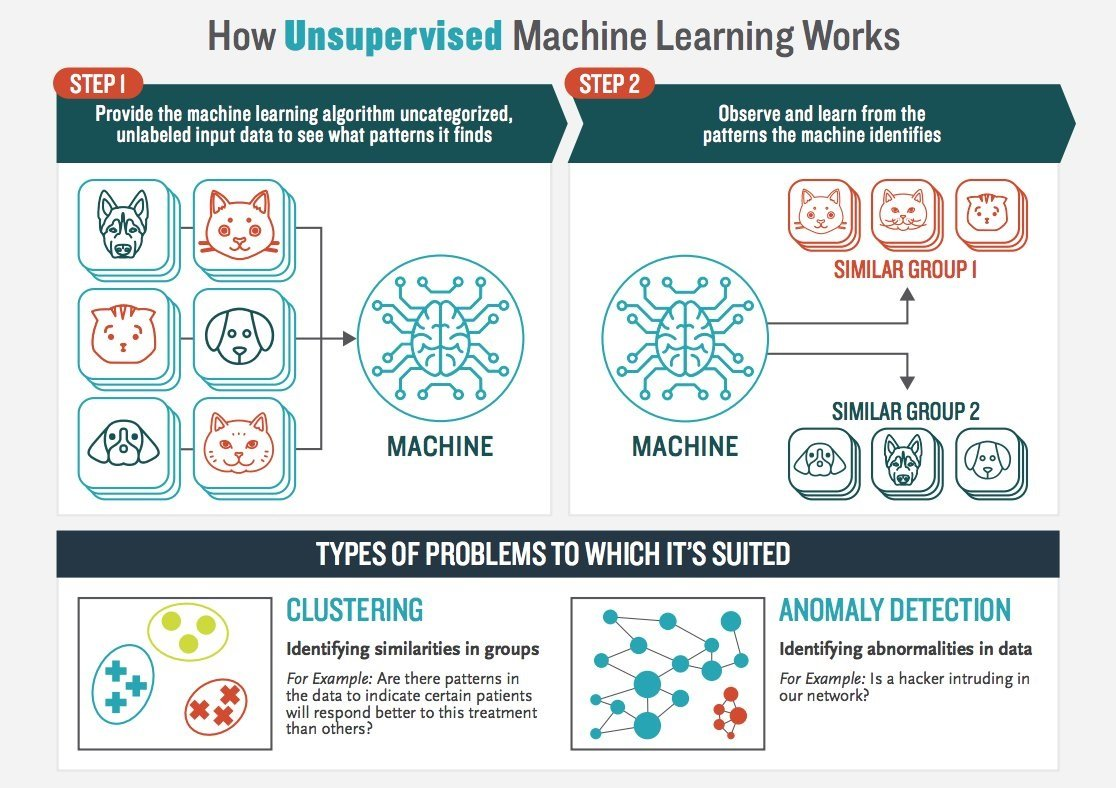
\includegraphics[width=1\textwidth]{figures/1184065/UnsupervisedLearning.jpg}
	\centering
	\caption{Unsupervised Learning}
\end{figure}
\item Data Set
\hfill\break
Data Set dapat dipandang sebagai kumpulan objek data. Dalam kasus data tabular, satu set data sesuai dengan satu atau bahkan lebih tabel database, yang dimana setiap kolom tabel mewakili variabel tertentu, dan setiap baris sesuai dengan catatan tertentu dari set data yang dimaksud.
\begin{figure}[h]
	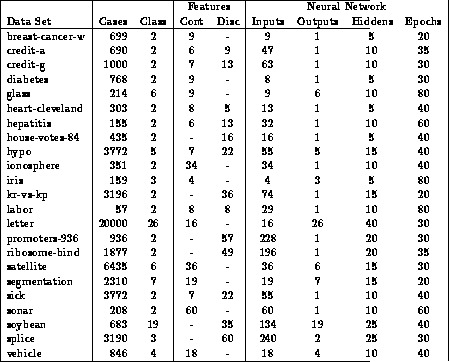
\includegraphics[width=1\textwidth]{figures/1184065/dataset.png}
	\centering
	\caption{Data Set}
\end{figure}
\item Training Set
\hfill\break
Training Set adalah bagian dataset yang kita latih untuk membuat prediksi atau menjalankan fungsi dari sebuah algoritma Machine Learning. Kita memberikan petunjuk melalui algoritma supaya mesin yang kita latih bisa mencari korelasinya sendiri atau juga bisa belajar pola dari data yang diberikan.
\item Testing Set
\hfill\break
Test set adalah bagian dataset yang kita test untuk melihat keakuratannya, atau dengan lkata lain melihat performannya.
\end{enumerate}
\end{enumerate}

\section{Instalasi}
Membuka https://scikit-learn.org/stable/tutorial/basic/tutorial.html. Dengan menggunakan bahasa yang mudah dimengerti dan bebas plagiat. 
Dan wajib skrinsut dari komputer sendiri.
\begin{enumerate}
\item
Instalasi library scikit dari anaconda, mencoba kompilasi dan uji coba ambil contoh kode dan lihat variabel explorer[hari ke 1](10)
\begin{enumerate}
\item Pertama-tama pastikan sudah menginstall Anaconda. Jika sudah menginstall Anacoda jalankan Anaconda pada Anaconda Navigator.
\begin{figure}[H]
	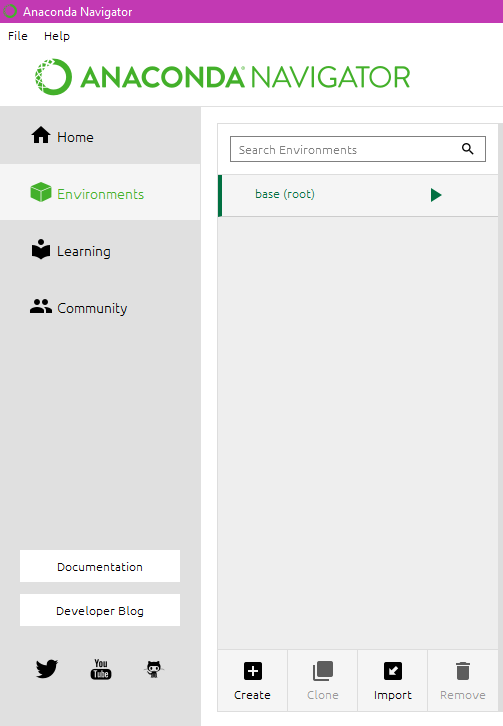
\includegraphics[width=1\textwidth]{figures/1184065/InstallLibraryScikit.png}
	\centering
	\caption{Installasi Library Scikit}
\end{figure}
\item Selanjutnya, klik menu Environment.
\item Kemudian klik environment base(root). Pada tahap ini akan melakukan installasi library scikit-learn di environment base(root).
\item Lalu pilih All. Untuk menampilkan list library yang ada.
\item Setelah itu cari scikit-learn di kolom pencarian.
\item Selanjutnya centang library scikit-learn lalu klik tombol Apply.
\begin{figure}[H]
	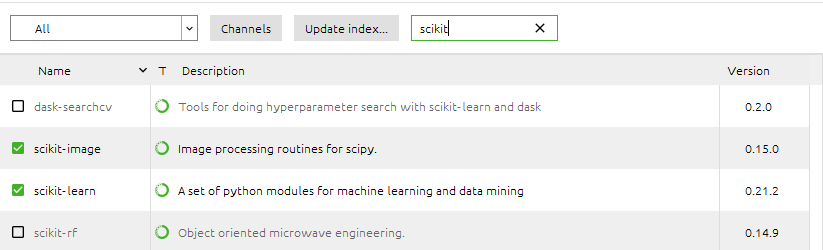
\includegraphics[width=1\textwidth]{figures/1184065/scikit-learn.png}
	\centering
	\caption{Installasi Library Scikit-Learn}
\end{figure}
\hfill\break
\textbf{Mencoba Menggunakan Library Scikit-Learn}
\begin{enumerate}
\item Pertama buka atau jalankan spyder.
\item Buat file baru, kemudian tambahkan kode seperti berikut ini.
\lstinputlisting[language=Python]{src/1184065/variable.py}
\item Simpan dan jalankan.
\item Hasilnya akan seperti berikut ini.
\begin{figure}[H]
	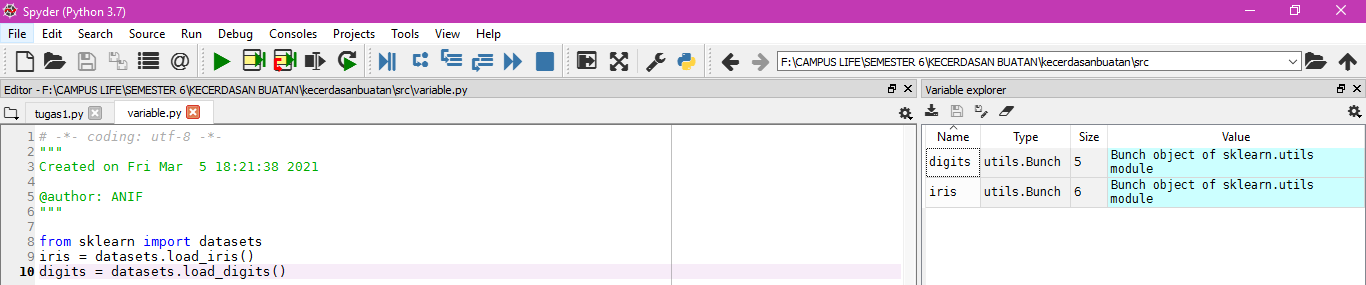
\includegraphics[width=1\textwidth]{figures/1184065/Variable.png}
	\centering
	\caption{Variabel Explorer Library Scikit-Learn}
\end{figure}
\end{enumerate}
\end{enumerate}
\item Mencoba Loading an example dataset, menjelaskan maksud dari tulisan tersebut dan mengartikan per baris[hari ke 1](10)
\lstinputlisting[language=Python]{src/1184065/soal2.py}
Kemudian jalankan, maka hasilnya akan seperti berikut ini.
\begin{figure}[H]
	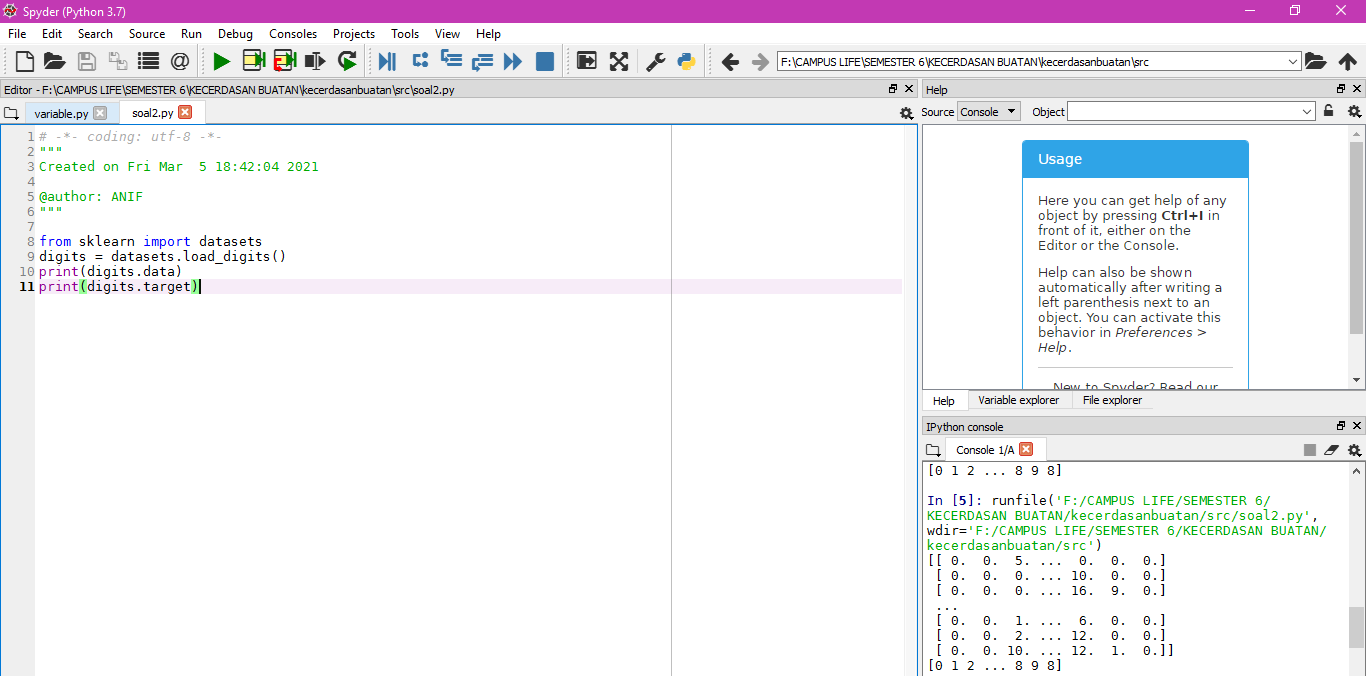
\includegraphics[width=1\textwidth]{figures/1184065/soal2.png}
	\centering
	\caption{Hasil Loading an Example Dataset}
\end{figure}
\hfill\break
Keterangan :
\hfill\break
Pada baris ke\-8 yaitu mengimport datasets dari library sklearn.
\hfill\break
Pada baris ke\-9 yaitu meload datasets digits yang kemudian akan ditampung pada variable digits.
\hfill\break
Pada baris ke\-10 yaitu menampilkan data dari datasets digits.
\hfill\break 
Pada baris ke\-11 yaitu menampilkan target dari datasets digits.
\item Mencoba Learning and predicting, menjelaskan maksud dari tulisan tersebut dan mengartikan per baris[hari ke 2](10)
\lstinputlisting[language=Python]{src/1184065/soal3.py}
Kemudian jalankan, maka hasilnya akan seperti berikut ini.
\begin{figure}[H]
	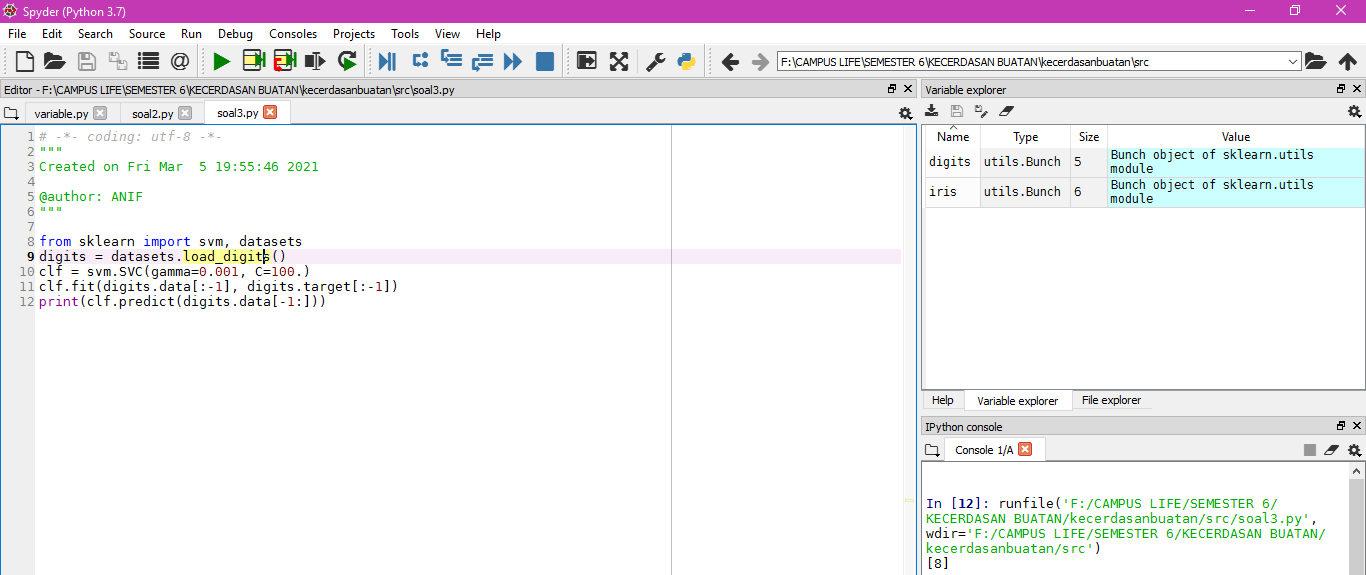
\includegraphics[width=1\textwidth]{figures/1184065/soal3.png}
	\centering
	\caption{Hasil Mencoba Learning and Predicting}
\end{figure}
\hfill\break
Keterangan :
\hfill\break
Pada baris ke\-8 yaitu mengimport svm dan datasets dari library sklearn.
\hfill\break 
Pada baris ke\-9 yaitu meload datasets digits dan ditampung di variable digits.
\hfill\break
Pada baris ke\-10 yaitu memanggil class SVC (Support Vector Classification)dan argument constructor SVC dan ditampung pada variable  clf.
\hfill\break
Pada baris ke-11 yaitu memanggil method fit untuk melakukan training data dengan argumen data dan target datsets.
\hfill\break
Pada baris ke-12 yaitu menampilkan hasil dari method predict dengan argumen data digits terakhir.
\item
Mencoba Model persistence, menjelaskan maksud dari tulisan tersebut dan mengartikan per baris[hari ke 2](10)
\lstinputlisting[language=Python]{src/1184065/soal4.py}
\begin{figure}[H]
	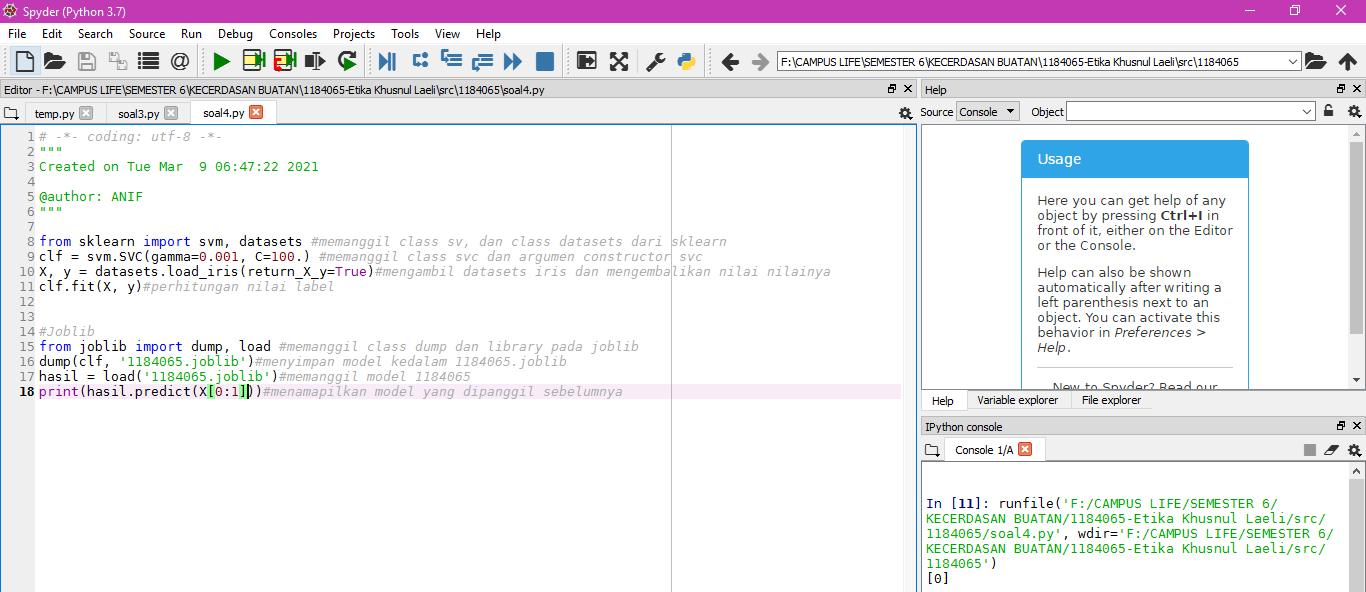
\includegraphics[width=1\textwidth]{figures/1184065/soal4.png}
	\centering
	\caption{Hasil Model Persistence}
\end{figure}
\item 
Mencoba Conventions, menjelaskan maksud dari tulisan tersebut dan mengartikan per baris[hari ke 2](10)
\lstinputlisting[language=Python]{src/1184065/soal5.py}
\end{enumerate}


\section{Penanganan Error}
Dari percobaan yang dilakukan di atas, apabila mendapatkan error maka:

\begin{enumerate}
	\item
	skrinsut error[hari ke 2](10)
	\begin{enumerate}
	\item Error 1
	\begin{figure}[H]
	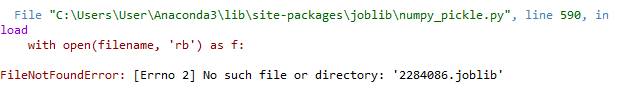
\includegraphics[width=1\textwidth]{figures/1184065/error1.png}
	\centering
	\caption{Import Error}
\end{figure}
\item Error 2
\begin{figure}[H]
	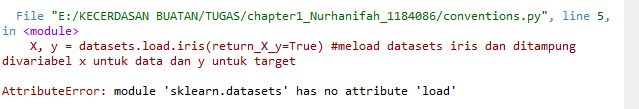
\includegraphics[width=1\textwidth]{figures/1184065/error2.png}
	\centering
	\caption{Name Error}
	\end{figure}
	\item Error 3
	\begin{figure}[H]
	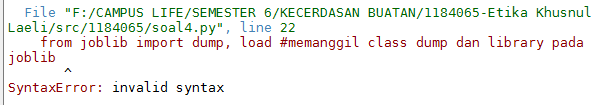
\includegraphics[width=1\textwidth]{figures/1184065/error3.png}
	\centering
	\caption{Syntax Error}
	\end{figure}
	\end{enumerate}
	\item
Tuliskan kode eror dan jenis errornya [hari ke 2](10)
\begin{enumerate}
\item Import Error yaitu error terjadi saat syntax melakukan import terhadap library yang tidak diketahui.
\item  Name Error yaitu error terjdi saat syntax melakukan eksekusi terhadap local name yang tidak terdefinisi.
\item Syntax Error yaitu Error yang terjadi karena kesalahan ketik.
\end{enumerate}
	\item
Solusi pemecahan masalah error tersebut[hari ke 2](10)
\begin{enumerate}
\item Solusi Import Error
\hfill\break
Solusinya yaitu memastikan library pada saat dipanggil itu ada dan tidak terjadi kesalahan ketik pada library.
\item Solusi Name Error 
\hfill\break
Solusinya yaitu memastikan variabel atau function yang dipanggil ada dan tidak sala ketik.
\item Solusi Syntax Error
\hfill\break
Solusinya yaitu memastikan tidak adanya kesalahan dalam pengetikan.
\end{enumerate}
\item Bukti bebas Plagiat
\begin{enumerate}
\item Bukti bebas plagiat 1
\begin{figure}[H]
	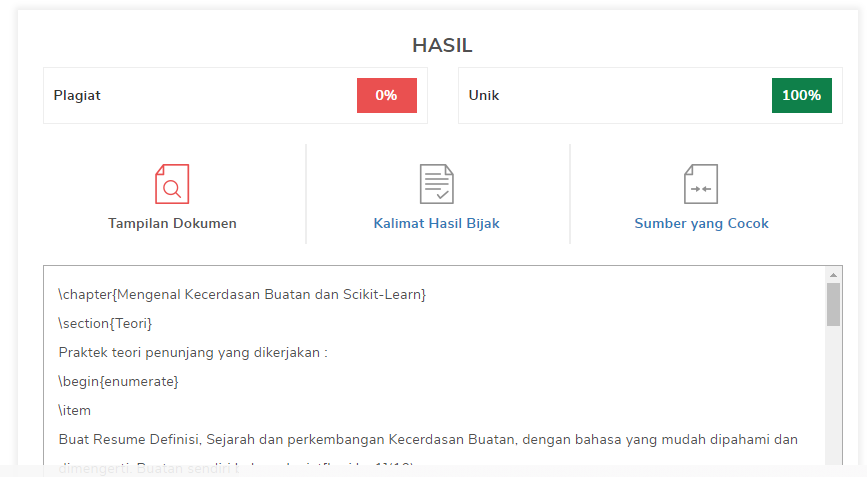
\includegraphics[width=1\textwidth]{figures/1184065/bukti1.png}
	\centering
	\caption{Bukti Bebas Plagiat 1}
	\end{figure}
	\item Bukti bebas plagiat 2
	\begin{figure}[H]
	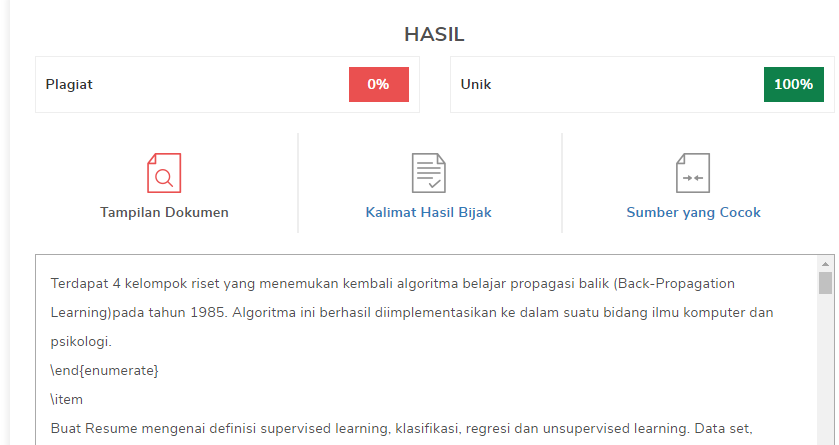
\includegraphics[width=1\textwidth]{figures/1184065/bukti2.png}
	\centering
	\caption{Bukti Bebas Plagiat 2}
	\end{figure}
\end{enumerate}

\end{enumerate}

